%Copyright 2014 Jean-Philippe Eisenbarth
%This program is free software: you can
%redistribute it and/or modify it under the terms of the GNU General Public
%License as published by the Free Software Foundation, either version 3 of the
%License, or (at your option) any later version.
%This program is distributed in the hope that it will be useful,but WITHOUT ANY
%WARRANTY; without even the implied warranty of MERCHANTABILITY or FITNESS FOR A
%PARTICULAR PURPOSE. See the GNU General Public License for more details.
%You should have received a copy of the GNU General Public License along with
%this program.  If not, see <http://www.gnu.org/licenses/>.

%Based on the code of Yiannis Lazarides
%http://tex.stackexchange.com/questions/42602/software-requirements-specification-with-latex
%http://tex.stackexchange.com/users/963/yiannis-lazarides
%Also based on the template of Karl E. Wiegers
%http://www.se.rit.edu/~emad/teaching/slides/srs_template_sep14.pdf
%http://karlwiegers.com
\documentclass{scrreprt}
\usepackage{listings}
\usepackage{underscore}
\usepackage[bookmarks=true]{hyperref}
\usepackage[utf8]{inputenc}
\usepackage[english]{babel}
\usepackage{longtable}
\usepackage{graphicx}
\graphicspath{ {./images/} }
\hypersetup{
    colorlinks=true,
    bookmarks=false,    % show bookmarks bar?
    pdftitle={Design Document},    % title
    pdfauthor={Jean-Philippe Eisenbarth},                     % author
    pdfsubject={TeX and LaTeX},                        % subject of the document
    pdfkeywords={TeX, LaTeX, graphics, images}, % list of keywords
    colorlinks=true,       % false: boxed links; true: colored links
    linkcolor=blue,       % color of internal links
    citecolor=black,       % color of links to bibliography
    filecolor=black,        % color of file links
    urlcolor=purple,        % color of external links
    linktoc=page            % only page is linked
}%
\def\myversion{1.0 }
\date{}
%\title
\usepackage{hyperref}
\begin{document}

\begin{flushright}
    \rule{16cm}{5pt}\vskip1cm
    \begin{bfseries}
        \Huge{SOFTWARE ARCHITECTURE}\\
        \vspace{1.9cm}
        for\\
        \vspace{1.9cm}
        GBUS Scheduling App\\
        \vspace{1.9cm}
        \LARGE{Version \myversion approved}\\
        \vspace{1.9cm}
        Prepared by Jack Doiron, Jared Cassarly, Shota Nemoto, Martin Peters\\
        \vspace{1.9cm}
        \today\\
    \end{bfseries}
\end{flushright}

\tableofcontents


\chapter*{Revision History}

\begin{center}
    \begin{tabular}{|c|c|c|c|}
        \hline
	    Name & Date & Reason For Changes & Version\\
        \hline
	    Jack Doiron & 2/22/19 & initial draft & 1.0 draft 1\\
        \hline
    \end{tabular}
\end{center}

\chapter{User Interface}

this section describes UI

\section{Home Screen}

talk about home

\section{Event Editing and Creation Menu}

event edit

\section{General Settings Menu}

settings

\section{Account Management}

The user can sign up for an account, login, logout, or reset their password.  The Sign Up UI should come up upon opening the app while not logged in and after signing out.

\subsection{Account Management Form Fields}
\begin{center}
\begin{longtable}{ | p{3cm} | p{4cm} | p{8cm} | }
\hline
\textbf{Field Name} & \textbf{Field Type} & \textbf{Description} \\
\hline
email & email address & the user's email address \\
\hline
password & password & password of the user \\
\hline
second password & password & second password field to verify the user's password\\
\hline
\end{longtable}
\end{center}

\subsection{Account Management Interfaces}
There are 3 user interfaces related to account management:\\
\textbf{Log In:}
logs the user in.  Uses the email and password fields.
\begin{center}
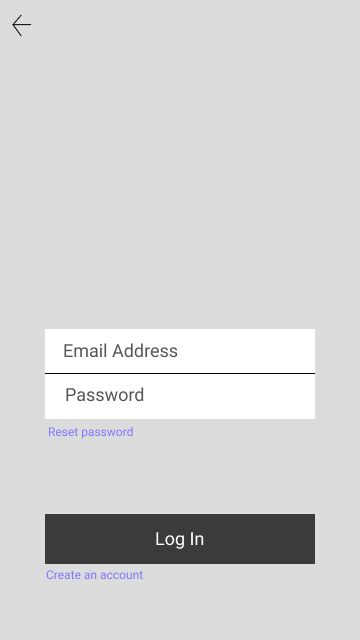
\includegraphics[scale=0.4]{login.png}
\end{center}

\textbf{Reset Password:}
Tells the server to send a reset password email.  Uses email field.
\begin{center}
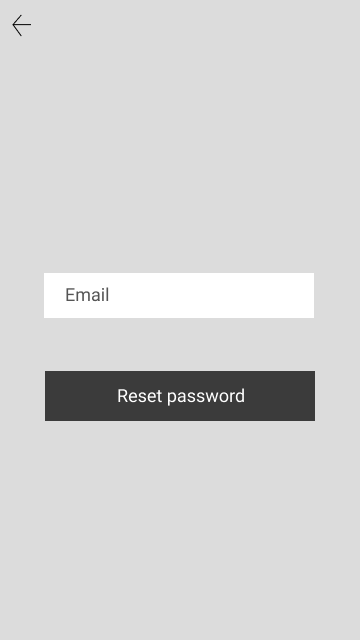
\includegraphics[scale=0.4]{resetpass.png}
\end{center}

\textbf{Sign Up:}
Requests the server to sign the user up.  Uses the email, password, and second password fields.
\begin{center}
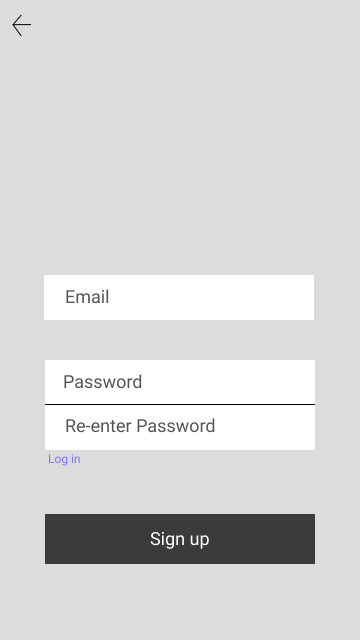
\includegraphics[scale=0.4]{signup.png}
\end{center}

\section{Auto Scheduler Diff View}

diff

\section{Toolbar}

toolbar

\subsection{Drag and Drop Events}

dragndrop

\subsection{Resize Events}

resize

\subsection{Cut/Copy/Paste}

copy pasta

\subsection{Create Event}

create

\subsection{Edit Event}

edit

\subsection{View Mode}

view

\chapter{Auto Scheduler}

\section{Description}
The Auto Scheduler implements the functionality described in section 4.2 of the Software Requirements Spec.  It must take in a full schedule and a deadline event.  It then returns either a new valid full schedule, or an error if the requested schedule is impossible.

\section{Input}
\begin{center}
\begin{longtable}{ | p{5cm} | p{9cm} | }
\hline
\textbf{Input Name} & \textbf{Input Type}\\
\hline
Old Schedule & Schedule \\
\hline
New Deadline Event & Deadline \\
\hline
\end{longtable}
\end{center}

\section{Output}
\begin{center}
\begin{longtable}{ | p{5cm} | p{9cm} | }
\hline
\textbf{Output Name} & \textbf{Output Type}\\
\hline
New Schedule & Schedule \\
\hline
\end{longtable}
\end{center}

\section{Behavior}
The new schedule must conform to the functional requirements specified in Section 4.2.3 of the Requirements Specification.

\chapter{Event Storage Classes}

classes

\chapter{Synchronization and Account}

\section{Description}
The server must allow a user to log in, log out, as well as sync their data to and from the server.

\section{Database}
The server must communicate with a database storing the following fields.
\begin{center}
\begin{longtable}{ | p{3cm} | p{4cm} | p{7cm} | }
\hline
\textbf{Field Name} & \textbf{Field Type} & \textbf{Description}\\
\hline
user id & uuid & A unique identifier for the user\\
\hline
email & email & The user's email address\\
\hline
verified & boolean & Is the user's email address verified?\\
\hline
verification token & string & string used to verify a user's email address\\
\hline
salt & string & unique random string to use while hashing the user password\\
\hline
password hash & string & the hash of the user's salted password\\
\hline
schedule & string or file reference & This field should contain either a serialized version of the user's
entire calendar schedule or a reference to a file containing such data.\\
\hline
\end{longtable}
\end{center}

\section{Events}
\subsection{Create Account}
\begin{center}
\begin{tabular}{ p{2cm} p{13cm} }
Description: & The Server receives a request to create a new account with an email and password\\
Behavior: & The server creates a new entry in the database with the user's email and a unique user id.  It must give the 
account a unique salt, and then add the user's salted and hashed password.  The schedule is left empty and
verified must initially be False.  It then stores a random verification token and sends an email to the specified
email address with a link containing the verification token and the user email.\\
Errors Handling: & If any operation fails when creating the account, no database entry should be created as to avoid half
filled database entries.  If the user's email already exists in the database, a new account must not be created.
\end{tabular}
\end{center}

\subsection{Verify email}
\begin{center}
\begin{tabular}{ p{2cm} p{13cm} }
Description: & The server receives a request to verify an email along with a verification token\\
Behavior: & The server searches for the account with that email in the database and if the verification token matches
the entry in the database, verified is set to true.  Otherwise, the server sends back a failure to the user.\\
\end{tabular}
\end{center}

\subsection{Log In}
\begin{center}
\begin{tabular}{ p{2cm} p{13cm} }
Description: & The server receives a log in request with the email and password of the user\\
Behavior: & The server verifies that the salted and hashed password match the database and logs the user in,
assigning them a unique session identifier.  Otherwise, the user receives a login error\\
\end{tabular}
\end{center}

\subsection{Log Out}
\begin{center}
\begin{tabular}{ p{2cm} p{13cm} }
Description: & The server receives a request to log out along with a session identifier\\
Behavior: & The server invalidates the user's session identifier\\
\end{tabular}
\end{center}

\subsection{Sync from}
\begin{center}
\begin{tabular}{ p{2cm} p{13cm} }
Description: & A logged in user requests to sync from the server\\
Behavior: & The server responds with the schedule database entry corresponding to the user's session id\\
Error Handling: & No user data may be sent if the session id is not valid\\
\end{tabular}
\end{center}

\subsection{Sync to}
\begin{center}
\begin{tabular}{ p{2cm} p{13cm} }
Description: & A logged in user sends the server new schedule data\\
Behavior: & The server replaces the user's schedule data in the database with the recieved data\\
Error Handling: & No user data may be modified if the session id is not valid\\
\end{tabular}
\end{center}

\chapter{Appendix A: Glossary}
%see https://en.wikibooks.org/wiki/LaTeX/Glossary

Auto-Scheduler - Creates events in advance of deadlines. Can move unlocked events around.
See section Auto Scheduling.\\
\\
Event - A block of time on the scheduler with characteristics such as start time, end time,
location, description, name, locked toggle, etc. (see Event functional requirements).\\
\\

\end{document}